\chapter{Makahiki and SGSEAM Evaluation}
\label{cha:evaluation}

This chapter describes the way I evaluated the Makahiki framework described in \autoref{cha:makahiki-design} and the SGSEAM method described in \autoref{cha:sgseam-design}. First, I describe the Real-world case studies of Makahiki instances realized in the Kukui Cup Challenges at the different organizations, followed by the detailed assessment of applying SGSEAM to Makahiki framework. The evaluation is to address:
(a) obtain insights about the strength and weakness of the Makahiki serious game framework, (b) obtain insights about the strength and weakness of SGSEAM serious game framework assessment method.

\section{Real-world Makahiki Instances Case Studies}

Makahiki, as a serious game framework for sustainability, had been used by different organizations to create multiple serious game instances targeting to educate and foster sustainable behavior among the communities. The first Kukui Cup Energy challenges at the University of Hawaii at Manoa (UHM) were held in 2011 for 3 weeks for over 1,000 first year students living in the residence halls. UHM subsequently held the second and third Kukui Cup Energy challenges in 2012 and 2014 for different first year students and different durations, for 9 months and 2 weeks respectively. Hawaii Pacific University (HPU) held their Kukui Cup Energy challenge in Fall 2012 and 2013 for about 200 students each year. An international organization called the East-West Center (EWC) held a Kukui Cup Energy and Water challenge for the international residents living in the residence halls. An Hawaii private school called Holy Nativity School (HNS) held a pilot Kukui Cup challenge for the elementary school students. 

\autoref{table:instances} lists these instances and their different requirements. The major requirements are differed in the duration of the challenge, population that could participate in the challenge, the type of resource such as energy or water, whether they have smarter meters installed, and type of web server hosting. Additional difference in requirements includes the type of the authentication for the participation, the differences in the game mechanics implementation. These differences will be described in the result chapter in more details.

\begin{table}[ht!]
  \centering
  \begin{tabular}{|p{0.12\columnwidth}|p{0.12\columnwidth}|p{0.12\columnwidth}|p{0.17\columnwidth}|p{0.07\columnwidth}|p{0.1\columnwidth}|}
    \hline
    \tabhead{Instances} &
    \tabhead{Duration} &
    \tabhead{Populations} &
    \tabhead{Resource} &
    \raggedright \tabhead{Smart meters} &
    \tabhead{Hosting} \\
    \hline
    UHM 2011 & 3 weeks & 1038 & Energy & \checkmark & Local \\
    \hline
    UHM 2012 & 9 months & 1067 & Energy & \checkmark & Cloud \\
    \hline
    UHM 2014 & 2 weeks & 1056 & Energy & \checkmark & Cloud \\
    \hline
    HPU 2012 & 3 weeks & 198 & Energy & \checkmark & Local \\
    \hline
    HPU 2013 & 3 weeks & 197 & Energy & \checkmark & Local \\
    \hline
    EWC 2012 & 2 weeks & 129 & Energy \& Water & \xmark & Cloud \\
    \hline
    HNS 2013 & 7 months & 10 & Energy & \xmark & Cloud \\
    \hline    
  \end{tabular}
  \caption{Makahiki Serious Game Instances}
  \label{table:instances}
\end{table}

The Makahiki instances deployed at these organizations have to meet these different requirements. The goal of the Makahiki framework is to minimize the effort in supporting the different requirements in various organizations. The real world case study of Makahiki is to look at the different requirements of these organizations, and the corresponding different configurations in the Makahiki framework to support such requirements. A more formal assessment of the strength and weakness of the Makahiki framework is described in the next section, by applying SGSEAM to Makahiki, which assessing the experiences of various stakeholders of the Makahiki framework.

\section{Applying SGSEAM to Makahiki}

This section describes in details the application of SGSEAM to assess the Makahiki framework in order to identified the strengths and weaknesses of both the Makahiki and the SGSEAM itself.

\subsection{SGSEAM Stakeholders in Makahiki}
The first step in SGSEAM assessment method is to identify the stakeholders in Makahiki. \autoref{table:eval-stakeholders} listed the identified stakeholders who use the Makahiki framework. 

\begin{table}[ht!]
  \centering
  \begin{tabular}{|p{0.2\columnwidth}|p{0.4\columnwidth}|p{0.3\columnwidth}|}
    \hline
    \tabhead{Stakeholder class} &
    \tabhead{Tasks} &
    \tabhead{Role} \\
    \hline
    Player &
    Participate in the Makahiki games &
    Students living in the residential halls\\
    \hline
    System admin &
    Install Makahiki software, monitor and scale the system, backup, patch maintenance &
    IT staffs\\
    \hline
    Game designer &
    Design the content, configure suitable games and mechanics &
    Challenge organizers\\
    \hline
    Game manager &
    Manage the game during the period of game play.&
    Challenge organizers\\
    \hline
    Game developer &
    Develop customization, extend and enhance the game and framework. &
    Makahiki developers \\
    \hline
  \end{tabular}
  \caption{SGSEAM Stakeholders}
  \label{table:eval-stakeholders}
\end{table}

\subsection {SGSEAM Approach for Makahiki}

The second step in SGSEAM is to determine the assessment approach. As described in SGSEAM, The assessment approaches is categorized into {\em in-vivo} and {\em in-vitro} assessments. The  {\em in-vivo} approaches, such as pre-post test, in-game surveys and post-hoc interviews, assess the real world instance of the game. The {\em in-vitro} approaches use in-lab experiments in a simulated environment. Different assessment approaches will have different levels of rigor or validity. When applying SGSEAM in Makahiki, I used the real world Makahiki instances as the in-vivo approaches which includes pre-post effectiveness study for player assessment, post-hoc interview for game administrator and game designer. 

In addition to real world instances assessment, I also implemented the in-vitro assessment approach using the in-lab experiments. In Spring 2013, Professor Philip Johnson at the Information and Computer Science Department of University of Hawaii used Makahiki to teach a course in serious game development. The students were seniors or graduate students majoring in computer science related fields. During the course, the students installed Makahiki, designed a serious game instance with Makahiki, and developed an enhancement to the Makahiki system.
The participation is voluntary. This is considered as an in-lab experiment since they are evaluating Makahiki in a class setting and using Makahiki in the development environments.

\autoref{table:eval-approaches} lists the SGSEAM approaches that are used to assess the strengths and weaknesses of Makahiki from different stakeholders' view.

\begin{table}[ht!]
  \centering
  \begin{tabular}{|p{0.17\columnwidth}|p{0.32\columnwidth}|p{0.42\columnwidth}|}
    \hline
    \tabhead{Stakeholder}&
    \tabhead{Assessment approaches} &
    \tabhead{Expected Outcomes} \\
    \hline
    \multirow{4}{*}{Player} & Pre-post effectiveness study &
    Determine effectiveness in energy literacy and resource usage reduction \\
    \cline{2-3}
      & Self-reported effectiveness survey &
	determine self-reported effectiveness in behavior change and awareness\\
    \cline{2-3}
    & Self-reported usability survey &
	Identify problem areas in game interface\\
    \cline{2-3}
     & Engagement metrics &
	Determine the extent of engagement\\
    \hline
    \multirow{2}{*}{System admin} & Post-hoc admin interview &
    \multirow{2}{0.42\columnwidth}{Determine strengths and weaknesses in system install and maintenance}\\
    \cline{2-2}
    & In-lab system admin study & \\
    \hline
    \multirow{2}{*}{Game designer} & Post-hoc designer interview \& log data analysis &
	\multirow{2}{0.42\columnwidth}{Determine strengths and weaknesses in facilitating the game design process} \\
	\cline{2-2}	
	& In-lab game design study & \\
    \hline
    \multirow{2}{*}{Game manager} & Post-hoc manager interview \& log data analysis & 
	 \multirow{2}{0.42\columnwidth}{Determine strengths and weaknesses in managing the game} \\
	\cline{2-2} 
	& In-lab game management study & \\
    \hline
    Game developer & In-lab game development study & 
        Determine strengths and weaknesses in developing system enhancement \\
    \hline
  \end{tabular}
  \caption{SGSEAM approaches}
  \label{table:eval-approaches}
\end{table}

The following sections describe the assessment approaches in details. 

\subsubsection{Player assessment}

Real-world Makahiki instances at the University of Hawaii at Manoa were used to study the player's experience with the Makahiki framework. There are over 1000 eligible players for each of these instances. They are the first year college student living in four similar structured resident halls in close vicinity. The games lasted for 3 weeks for the year 2011 instance, 9 months for 2012 instance and 2 weeks for 2014 instance respectively. 

To assess the effectiveness of the framework for designing games that improve player literacy in sustainability, we
conducted two energy literacy surveys, one before the challenge (pre-game) and one after
the challenge (post-game). SurveyGizimo is used to create the surveys which consists of the set of sustainability literacy and behavior questionnaires. The response from the two surveys are analyzed to provide insights about the player's literacy and behavior change.

To assess the effectiveness of the framework for designing games that produce positive change in sustainability
behaviors, we recorded and analyzed energy consumption data before, during and after the
challenge.  Before the challenge, an energy usage baseline was established. The energy consumption data is examined to understand any usage pattern or reduction during and after the challenge. 

We also conducted the in-game self-reported behavior changes survey. The survey asked the questions about their interests in sustainability prior to and after the game, as well as any perceived behavior changes when playing the game.

To assess the usability of the game produced by the Makahiki framework, we conducted the in-game usability survey. The survey asked the questions about the players' experience about the user interface of the game. The response from the survey is analyzed to provide insights about the game usability.

In addition to the surveys and energy data measurement, the following engagement metrics is calculated based on the game and log data to assess the engagement level of the instance:

\begin{itemize}
\item participation rate
\item number of players per day
\item Play time per day
\item Submissions per day
\item Social interactions per day
\item Website errors per day
\end{itemize}

Besides the pre-post  and in-game survey response data, the following data recorded by the Makahiki system were used to assess player's experiences:
\begin{itemize}
\item energy data for each team before, during, and after the game.
\item game participation and submission data
\item logging data of every interaction between the players and the website.
\end{itemize}

\subsubsection{System admin assessment}

There are two approaches described in SGSEAM to assess the system admin's experience: One is the in-lab experiments, another is the interview of the system admin of a real world instance.

In the in-lab experiments, the students in the ICS691 Spring 2013 class were tasked with installing the Makahiki system into their local computers as well as the cloud environment. In order to understand how much time it takes to install the Makahiki and what problems might be encountered, I design a Google form which details the steps of installing Makahiki both locally and in the cloud, and for each step, I ask the students to record the time they spent and the problems they encountered.

\autoref{fig:developer-eval-form} illustrates a partial google form used for Makahiki system admin assessment. \autoref{app:googleform} includes the complete google form.
\begin{figure}[ht!]
   \centering
   \includegraphics[height=30em,width=30em]{developer-eval-form.eps}
   \caption{Makahiki Developer assessment Form}
   \label{fig:developer-eval-form}
\end{figure}

The students were also asked to provide feedback about their installation experiences in the form of blog post. In the blog post, I ask them to discuss the following topics:
\begin{itemize}
\item What is the most difficult step during installation?
\item What problems did you encounter during the installation?
\item Have you install any database, web server or similar server products prior to this assignment? Are those installations for development or production purpose?
\item If you have experience installing other servers before, How does your prior experience of installing other servers compare to the installation of Makahiki?
\item What could be improved about the Makahiki installation process?
\item Compare your experience of installing Makahiki in Heroku with installing it locally,
\end{itemize}

The qualitative data collected from the google form response and the blog post from the students will be analyzed to gain insights into how easy it is to install Makahiki, and what contributes to the efficiency of the installation.

In order to gain insights on the experience of a real world system admin who uses the Makahiki, I performed interviews to the system admins of the 2012 Hawaii Pacific University (HPU) challenges.

I analyzed qualitative data collected from the interviews and email changes. The data include:
\begin{itemize}
 \item time taken to install the Makahiki
 \item time taken to maintain the Makahiki, such as backup, monitoring
 \item problems encountered
\end{itemize}

\subsubsection{Game designer assessment}

There are also two approaches described in SGSEAM to assess the game designer's experience: One is the in-lab experiments, another is the interview of the game designer of a real world instance.

The students in the in-lab experiments were tasked to design a Kukui Cup like serious game using Makahiki. I designed another google form to ask students to follow the designing steps and record their time and problem encountered during their designing process. \autoref{app:googleform} has the complete google form for the steps the students need to follow.

The students were asked to provide feedback about their installation experiences in the form of blog post to discuss the following topics:
\begin{itemize}
\item What is the most difficult step during Challenge Design?
\item What problems did you encounter while designed the challenge?
\item What problems did you encounter while managing the challenge?
\item What could be improved for the Makahiki Challenge Design process?
\item What could be improved for the Makahiki Challenge Management process?
\end{itemize}

I performed interviews to the real world game designers of the 2012 Hawaii Pacific University challenge and the 2012 East West Center challenge. We asked them about his game designing experiences using the Makahiki game design admin
 interface.

I analyzed both the qualitative data collected from the interviews and email changes with the game designers, and the quantitative collected from the admin interface log data. The qualitative data includes:
\begin{itemize}
    \item How much time did you spend to configure the challenge global settings?
    \item how much time did you spend to setup the player data?
    \item how much time did you spend to design the individual games?
    \item What problem did you encountered?
    \item Did you find it difficult to configure? what is difficult?
    \item Did you find it difficult to design a specific game? which one, what is difficult?
    \item What did you like the least when using the system?
\end{itemize}

The quantitative data includes:
\begin{itemize}
 \item time taken to configure the challenge with regarding to different designing tasks
 \item problems encountered in the log file
\end{itemize}

\subsubsection{Game manager assessment}
I performed interviews to the real world game managers of the 2012 Hawaii Pacific University challenge and 2012 East West Center challenge to study the experience of the game management using Makahiki.

I analyzed both the qualitative data collected from the interviews and email changes with the game managers, and the quantitative collected from the admin interface log data. The qualitative data includes:
\begin{itemize}
\item How much time did you spend to approving the action submissions?
\item How much time did you spend to monitoring the game status?
\item How much time did you spend to notifying prize winners?
\item What problem did you encountered?
\item Did you find it difficult to manage? what is difficult?
\item What did you like the least when using the system?
\end{itemize}

The quantitative data include:
\begin{itemize}
 \item time taken to manage the challenge with regarding to different managing tasks
 \item problems encountered in the log file
\end{itemize}

\subsubsection{Developer assessment}

I performed the in-lab game development study with the students participated in the ICS691 serious game development class. The students in the experiment are tasked with developing an enhancement to the Makahiki instance. This involves setting up the development environment, following the tutorial to create the "Hello world" widget using Makahiki, and finally, develop an enhancement which extends the functionality of the Makahiki system. The enhancement is specified in 5 development tasks. 

The students are asked to submit their development source code to the public source code repository (Github) and write a blog post to discuss their efforts to complete the development activity.

I reviewed their source code to compare their code to the reference implementation, analyze the blog post from the students, as well as any email correspondence from students discussing problems during the development.

The students were asked to provide feedback about their development experiences in the form of blog post to discuss the following topics:
\begin{itemize}
\item What part is complete?
\item What part is not complete?
\item Which parts you found easy or hard to complete?
\item What problems did you encounter while developing this enhancement tasks?
\item What is your recommendations for the framework to improve development supports.
\end{itemize}

\subsection{Assessment Participants}

After the assessment approaches are determined, the next step in SGSEAM is to identify the assessment participants for the different stakeholders. \autoref{table:participants} lists the participants for assessing the Makahiki framework using SGSEAM. 

\begin{table}[ht!]
  \centering
  \begin{tabular}{|p{0.2\columnwidth}|p{0.45\columnwidth}|p{0.2\columnwidth}|}
    \hline
    \tabhead{Stakeholder class} &
    \tabhead{Person(s)} &
    \tabhead{Organization} \\
    \hline
    Player &
    All eligible players in the UH KC instance &
    UHM \\
    \hline
    System admin &
    ICS691 students, \newline system admin for HPU instance &
    UHM, HPU\\
    \hline
    Game designer &
    ICS691 students, \newline game designer for HPU  \& EWC instance &
    UHM, HPU, EWC \\
    \hline
    Game manager &
    ICS691 students, \newline game manager for HPU \& EWC instance &
    UHM, HPU, EWC \\
    \hline
    Game developer &
    ICS691 students &
    UHM\\
    \hline
  \end{tabular}
  \caption{SGSEAM Stakeholders}
  \label{table:participants}
\end{table}

\subsection{Assessment Data Collection and Analysis}

The SGSEAM assessment process for Makahiki is carried out by implementing the different assessment approaches for the stakeholder participants, both in real world Makahiki instances and in-lab experiments. The data collected from all the different assessment approaches includes:

\begin{itemize}
\item pre-post surveys from players
\item in-game usability survey from players
\item interviews audio recordings from system admin, game designers, game managers
\item email communications from system admin, game designers, game managers
\item website logs and errors
\item google forms results reported from in-lab experiment evaluation
\end{itemize}

The data is analyzed according to the assessment approach to determine the strengths and weaknesses of the Makahiki framework with the respects of the different stakeholders in questions.

\section{Consents from Human Research Study Subjects}
This research interviewed and studied the behaviors of several human subjects including:

\begin{itemize}
\item First year students who played the real world UHM Kukui Cup instances for 2011, 2012 and 2014
\item Students who participated in the UHM ICS691 in-lab experiment study
\item Administrators who used Makahiki to install, design, and manage the real world Kukui Cup instances in HPU and EWC
\end{itemize}

We had obtained their consents to participate into this research from all the above human subjects. The study is also approved by Office of Research Compliance at the University of Hawaii Human Studies Program under the CHS \#20451.

\section{Limitations}

There is limitation to this evaluation design. SGSEAM is designed to assess any serious game framework from the five major serious game stakeholder's perspectives. We only apply SGSEAM to one serious game framework, Makahiki, which is also designed by us. There is many internal knowledge of Makahiki that may affect the design of the SGSEAM, which some of the assessment approaches might not be effective in assessing other serious game framework. \autoref{future:other-framework} describes another serious game framework that is a good candidate to be applied with SGSEAM. 

Without another data point of the application of SGSEAM, there is not enough confidence in the evaluation of the SGSEAM itself. 

One limitation in the application of SGSEAM to Makahiki is the small numbers of sample in the post-hoc interview approach. Due to the nature of the this kind of serious game, it is common to have just one or two system admin(s), game designer(s), and game managers(s). It is often the case that the game designers are the same as the game managers. In our evaluation design, although there are 7 Makahiki game instances in 4 organizations, we can only interview 1 system admin from HPU instance, 3 game designers who is also game managers from HPU and EWC instances. The UHM instances were designed and managed by ourself. We also installed and deployed the instances except the HPU ones, so there is no other sys admin candidate.  

Given this limitations, the application of SGSEAM to Makahiki still resulted in useful insights into the strengths and weaknesses of the Makahiki framework.

\section{Summary}

This chapter described the evaluation design for both Makahiki and SGSEAM.  Makahiki, as a serious game framework for sustainability, had been used by different organizations to create multiple serious game instances targeting to educate and foster sustainable behavior among the communities. The real world case study of Makahiki is to look at the different requirements of these organizations, and the corresponding different configurations in the Makahiki framework to support such requirements. A more formal assessment of the strength and weakness of the Makahiki framework is to apply SGSEAM to Makahiki.

According to the SGSEAM guide, the assessment participants were identified by the categories of five SGSEAM stakeholders. The assessment approaches were determined. The {\em in-vivo} assessment approaches of pre-post effectiveness study, in-game surveys and post-hoc interviews were applied to the real-world Kukui Cup challenges created by the Makahiki framework, to assess the experiences of players, system admins, game designers, and game managers. The {\em in-vitro} assessment approaches of in-lab study used the UHM ICS691 serious game course to assess the experiences in game installation, game design and game development. After the assessment is carried out, the Makahiki strengths and weaknesses are compiled in the result report and the suggestion are input into the improvement action report. 
